%
% T�TULO DEL CAP�TULO
%
\chapter[PCM]{
	Point Cloud Manager
	\label{chapter_5}
}

\textbf{PCM} is a set of software tools and libraries that allow the user to manage massive point clouds. It comprises a new point cloud format, a multi-resolution spatial structure, a cache system and an external interface. 

\section[Design]{Design}

\begin{figure}[h]
	\centering
	%\includegraphics[scale=0.7]{/Users/osurfer3/Dropbox/PFC/Memoria/pfc/eps/kd_tree.eps}
	\caption[k-d tree]{
		Bounding box splitting process.
	}
	\label{kd_tree}
\end{figure}

\section[Memory hierarchy]{Memory hierarchy}

One of the principal concepts in PCM is the memory hierarchy management, that is made up of two levels of cache. When it is known that the data that is going to be used is related in some way and the different access types, software caches can yield substantial improvements in the performance of the system. In this case, we work mainly with geometric information obtained from real environments and the cache hierarchy will allow us to exploit the spatial coherence in the data.  

In this project, a cache system with two levels has been implemented. It will take care of the data transfer needs between memory levels (HDD - RAM - VRAM). This system will take into account the spatial relation between the data, and will have an architecture that will not only allow to store datasets in a HDD but anything with a filesystem (e.g. NFS from a network).

\begin{figure}[h]
	\centering
	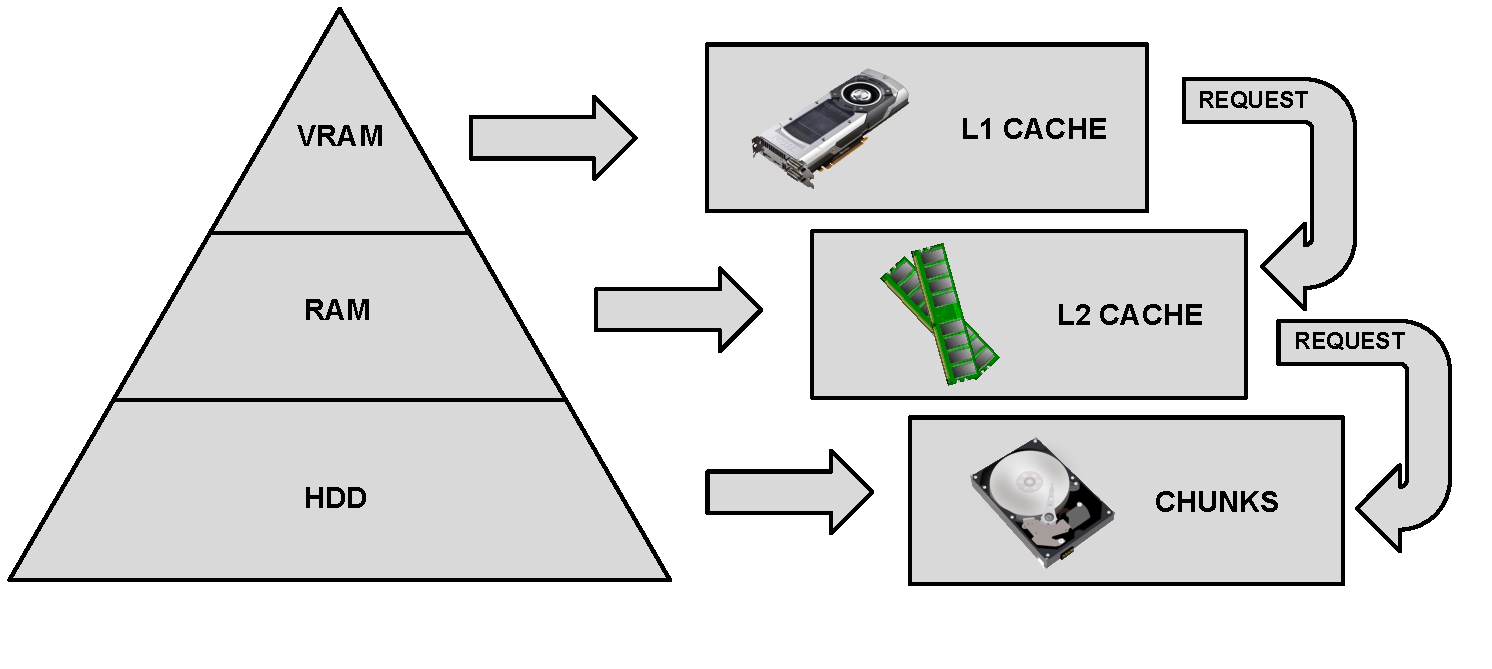
\includegraphics[scale=0.5]{figures/mem_hierch.pdf}
	\caption[Memory hierarchy]{
		Memory hierarchy of PCM.
	}
	\label{mem_hier}
\end{figure}

Between these three levels of memory will circulate the minimum unit of information, the chunk. A chunk is a ``container'' of a data subset, in our case points and data related to them.

The three levels are:

\begin{itemize}
	\item \textbf{Video memory or VRAM:} Volatile memory and less capacity than the next level, but even faster. Only the GPU will use this type of memory. The L1 cache will be created in this memory level.
	\item \textbf{Primary memory or RAM:} Volatile memory and low capacity compared to the next level, but fast. The CPU will use this type of memory. The L2 cache will reside in this cache level. 
	\item \textbf{Secondary memory or HDD:} Persistent memory and high density, but slower than the other two levels. In this level of memory will reside the point database.  
\end{itemize}  

First, in the lowest level, reside the binary files of each chunk. In the next level, RAM memory, a subset of chunks will be stored. Finally in VRAM, the chunks are adapted to a video memory compatible format, so that the GPU can work with them. 

These concepts will be further explained in the next subsections. 

\subsection[L1]{Synchronous cache L1}

The first level cache (L1) is in charge of managing the storing and loading of data between primary memory (RAM) and video memory (VRAM). This cache level has been completely reworked, and also has been given the ability to not only load but also store information in primary memory. Even having a similar structure to the L2 cache, because of the characteristics of GPU processes, its operation is synchronous. 

Its biggest responsibility, apart from the corresponding memory hierarchy management, will be the conversion of chunks of data to \textit{VBOs}\footnote{\textit{Vertex Buffer Object}: Structure that allows to store arrays of data in video memory.} in VRAM and viceversa. A chunk may have to be broken up into several VBOs depending on its size, so that optimal sizes of VBOs can be maintained for the GPU.

\begin{figure}[h]
	\centering
	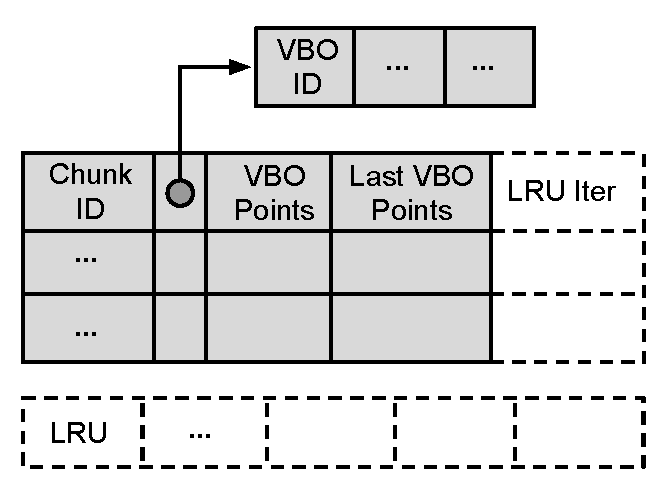
\includegraphics[scale=0.7]{figures/l1_cache.pdf}
	\caption[L1 cache structure]{
		L1 cache structure.
	}
	\label{l1_cache}
\end{figure}

The following list will explain each of the fields that make up the cache structure:

\begin{itemize}
	\item \textbf{Chunk ID:} Id of the chunk stored in L1 cache.
	\item \textbf{VBO ID:} IDs of the VBOs used to store points in the L1 cache entry.
	\item \textbf{VBO Points:} Number of points stored in all but the last VBO in the cache entry.
	\item \textbf{Last VBO Points:} Number of points in the last VBO in the cache entry.
	\item \textbf{LRU Iter:} Iterator to cache entry in LRU access record for fast updating of LRU.
	\item \textbf{LRU:} Least Recently Used chunk. 
	\item \textbf{Write:} Flag that marks chunk for storing. 
\end{itemize} 

Also two replacement policies were implemented:

\begin{itemize}
	\item \textbf{Naive:} Erase any data block that is not necessary looping over the complete cache one time. This method does not take into account when was the last time that a block was last used, if it is not necessary it will be erased. 
	\item \textbf{LRU\footnote{\textit{Least Recently Used}}:} This algorithm, will replace the elements that have been used least recently if the cache is full. If not full it will keep inserting nodes until it is.  
\end{itemize} 

To store the list of nodes currently in the cache two STL\footnote{\textit{Standard Template Library}} data structures can be used:

\begin{itemize}
	\item \textbf{Map:} An associative container with key-value pairs with ordered unique keys. Complexity of searches and element access is logarithmic in size: $O(\log n)$. 
	\item \textbf{HashMap:} It also contains key-value pairs with unique keys but without an order, element access is done using a hash function. Complexity of searches and element access is constant in the average case: $O(1)$ and linear in size in the worst case: $O(n)$.
\end{itemize}

Either of these two structures will meet our objective of making cache searches fast, as this is a crucial function that will be frequently used. Theoretically the use of one or the other depends on the number of nodes that the cache will contain. A Map will be faster with less elements, while the HashMap will be faster with big quantities of nodes. 

Another implemented feature are types of cache requests, there are several available:

\begin{itemize}
	\item \textbf{Restricted by time:} In order for the render process to be interactive and that no freezes occur, we will limit loading of VBOs by time. This type of petition will be limited by the time that the user desires (e.g. 3 ms). The cache will load as much nodes as possible in the given time and if the maximum time is reached it will stop loading nodes, even if there are still nodes missing. 
	\item \textbf{Restricted by level:} This type of request is usually used in GPGPU calculations, where no interactivity is needed. The user will specify a level of precision and the cache will load as many nodes as necessary for that level of detail.
\end{itemize}

This cache not only can read and load nodes from L2, it also has the ability to store changes made in video memory (L1) in RAM (L2). The user can choose if he wants the changes made in GPU (e.g. an OpenCL kernel) to be persistent or not.

When the node is evicted from the cache, its changes will be written to the L2 cache prior to its deletion. In the \autoref{l1_write} we not only show how to write changes to other cache levels, but also how to use PCM with its new \textbf{\textcolor{Emerald}{PointCloud}} interface to loop over the complete cloud out of core and perform some custom operation.

This process is completely transparent for the user, that will only have to use this example code:
\\
\lstset{language=C++,frame=shadowbox,rulesepcolor=\color[gray]{0.8},lineskip=10pt, 
		keywordstyle=\color{VioletRed}\bfseries,
		emph={PointCloud}, emphstyle=\color{Emerald}\bfseries,
		emph={[2]setChunkWriteL1,getNextDataGPU,getL1Entry,makeChangesGPU}, emphstyle={[2]\color{PineGreen}},label={l1_write} }
\begin{lstlisting}
 PointCloud cloud(...);

 while (cloud.getNextDataGPU(list)) {
 	for (auto& node:list) {		
		auto * VBOdata = cloud.getL1Entry(node);
		if (VBOdata) {
			makeChangesGPU(node);
			cloud.setChunkWriteL1(node);
		}		
	}
 }
\end{lstlisting}

\subsection[L2]{Asynchronous cache L2}

The second level cache L2, will be in charge of transferring data (chunks) from disk to system memory (RAM). The replacement policy used in this cache is LRU \cite{taibo} as this is the most adequate policy for these types of systems. 

To better use the resources available nowadays (multi-core CPUs), this cache will run on its own thread. Also since the massive datasets that we will deal with require a lot of computational power for even the simplest operations, this cache will be prepared to deal with simultaneous requests from different work threads. All of this is achieved with careful use of \textit{mutex}\footnote{A synchronization mechanism for enforcing limits on access to a resource in an environment where there are many threads of execution.} and \textit{semaphores}\footnote{A variable or abstract data type that is used for controlling access, by multiple processes, to a common resource in a parallel programming or a multi user environment.}. 

This cache is also capable of not only reading data from the HDD, but is also capable of writing modified data from RAM to disk. This is achieved in a similar fashion as in L1. A complete loop over the whole cloud to perform an operation using the CPU can be seen in \autoref{l2_write}.

\lstset{emph={PointCloud,Chunk}, emphstyle=\color{Emerald}\bfseries,
		emph={[2]setChunkWriteL2,getNeighborData,getChunkL2,makeChanges,freeChunkL2}, emphstyle={[2]\color{PineGreen}},label={l2_write}}
\begin{lstlisting}
 PointCloud cloud(...);

 while (cloud.getNeighborData(list)) {
 	for (auto& node:list) {		
		Chunk c;
		cloud.getChunkL2(node, c);
		makeChanges(c);
		cloud.setChunkWriteL2(node);	
		cloud.freeChunkL2(node);	
	}
 }
\end{lstlisting}

\subsection[Chunks]{Chunks}
\subsection[Chunks]{PCMBenchmark}